
\section{Analysis strategy}
\label{sec:analysis}

In section we describe our analysis strategy, and in particular
the classification of each individual event into
different categories according to its topology.
%
First of all we discuss the settings and nomenclature that
we will use for jet clustering, and then we move to discuss how $b$-tagging is simulated.
%
Then we discuss the categorisation of events between different
topologies, and how we prioritise among them.
%
Finally, we motivate our choice of analysis cuts by comparing signal and background
for the relevant kinematic distributions.

\subsection{Jet reconstruction}

The starting point after the parton shower is the clustering
of all final state particles using the
jet reconstruction algorithms
are obtained from the {\tt FastJet} program~\cite{Cacciari:2011ma},
v3.1.0.
%
In our study use different types of jet definitions,
which we enumerate now:
%

\begin{itemize}
\item {\it Small-$R$ jets}.

  These are jets  reconstructed with the
  anti-$k_T$ clustering algorithm~\cite{Cacciari:2008gp} with $R=0.4$ radius.
  %
  When reconstructing small-$R$ jets, we keep only
  those jets with transverse momentum $p_T \ge 40$~GeV
  and pseudo-rapidity $|\eta|<2.5$ within the central
  acceptance of ATLAS and CMS.
%
  Jets that fail to satisfy these acceptance
  requirements are discarded.
  %
  The restriction to the central rapidity region is a
  requisite for $b$-tagging.
    

\item {\it Large-$R$ jets}.

  These jets are also constructed with the
  anti-$k_T$ clustering algorithm, now using a $R=1.0$ radius.
  %
  In order to be accepted, these large-$R$ jets should
  satisfy  $p_T \ge 200$~GeV and lie in a pseudo-rapidity range by
  $|\eta|<2.0$.
  %
  If these conditions are not satisfied, the jet is discarded.
  %
  The more restrictive range  in pseudo-rapidity
  as compared to the small-$R$ jets
  is motivated by mimicking the  experimental requirements
  in ATLAS and CMS
  related to the track-jet-based calibration~\cite{Aad:2014bia,ATLAS:2012kla}.

  In addition to the basic $p_T$ and $\eta$
  acceptance requirements, large-$R$ jets should also
  satisfy the  BDRS mass-drop tagger~\cite{Butterworth:2008iy}
  conditions, in order
  to enhance the discrimination of the signal over the background
  events.
  %
  For the BDRS mass-drop tagger, we use the {\tt FastJet} default
  parameters of  $\mu = 0.67$ and $y_{\textrm{cut}}= 0.09$.
  %
  As required, before the mass-drop tagger is applied, the large-$R$ jet
  constituents are reclustered with the Cambridge/Aachen
  algorithm~\cite{Dokshitzer:1997in,Wobisch:1998wt}.

  
\item {\it Small-$R$ subjets}.

  Once we have reconstructed a suitable large-$R$ jet, important
  information can be obtained by looking at the kinematics of
  the small-$R$ subjets.
  %
  These subjets will be obtained by reclustering the constituents
  of the large-$R$ jet, always with the  anti-$k_T$ algorithm,
  but this time with a smaller radius parameter $R=0.3$.
  %
  These small-$R$ subjets will be the input of
  the $b$-tagging in the boosted category.
  %
  Small-$R$ subjets are required to have $p_T > 50$~GeV and $|\eta|<2.5$,
  else they are discarded.
  %
\end{itemize}

Let us mention that we explored the possible improvements
in the analysis from using variable-$R$ jets~\cite{Krohn:2009zg}, but found that these made
a small difference as compared to fixed-$R$ jets.
%
This is not unexpected, since variable-$R$ jets are more suitable when
the degree of boost of the final state being reconstructed can span
a wide range, such as in heavy resonance searches~\cite{Aad:2015fna}.


\subsection{$b$-tagging}

Given the $4b$ final state that needs to be reconstructed, the
optimisation of the $b$-tagging capabilities of the
LHC experiments is an essential requirement to improve
the prospects for the observation of Higgs pair production in this channel.
%
The $b$-tagging used in this feasibility study is inspired
in the current and projected ATLAS settings~\cite{Aad:2013gja},
though
it is not too different from
 the corresponding CMS strategy~\cite{Khachatryan:2011wq,Chatrchyan:2012jua}.
%
For each type of jet defined above, a different
$b$-tagging strategy is used:

\begin{itemize}

\item {\it Small-$R$ jets}.

  These are $b$-tagged as follows.
  %
  If a small-$R$ jet has at least one $b$-quark among their constituents,
  it will be tagged as a $b$-jet with probability $f_b$.
  %
  In order to be considered in the $b$-tagging algorithm,
   $b$-quarks should satisfy $p_T \ge 15$ GeV.
  %
  If no $b$-quarks are found among the constituents
  of this jet, it can be still be tagged as a $b$-jet with
  a mistag rate of $f_l$.
  %
  The probability of tagging a jet is not modified
  if more than one $b$-quark is found among the jet constituents.

  We only attempt to $b$-tag the four (two) hardest small-$R$ jets
  in the resolved (intermediate) category.
  %
  We find that
  attempting to $b$-tag all
  small-$R$ jets that satisfy the acceptance cuts worsens the performance
  due to combinatorics after the parton shower.

  \item {\it Large-$R$ jets}.

    Large-$R$ jets are $b$-tagged by
    ghost-associating anti-$k_T$ $R=0.3$
    subjets to the original large-$R$
    jets~\cite{Cacciari:2007fd,Aad:2013gja,
      ATLAS-CONF-2014-004}.\footnote{The same
    method was used in the recent ATLAS $hh\to 4b$ search~\cite{Aad:2015uka}.}
    %
    In particular,
    a large-$R$ jet is considered  double-$b$-tagged if both
    the leading and subleading subjets (where the ordering
    is done in the subjet $p_T$) are both individually $b$-tagged.
    %
    As in the case
    of small-$R$ jets, in
    order to be considered in the $b$-tagging algorithm,
   $b$-quarks should satisfy $p_T \ge 15$ GeV.
    %
    Note that we only attempt to $b$-tag the two leading subjets:
    trying to $b$-tag all subjets above the $p_T$ cut degrades
    the signal significance due to the increase in combinatorics.

    Concerning the $b$-tagging probabilities and the
    light jet mistag probabilities, there are taken
    the same as for small-$R$ jets.
    %
    Therefore, a large-$R$ jet where the two leading
    subjets have at least one $b$-quark will be tagged
    with probability $f_b^2$, if only one of the two leading
    subjets has a $b$-quark then the tagging probability is
    $2f_bf_l$, and if none of the two have $b$-quarks
    as constituents, the mistag rate will be
    $f_l^2$.


\end{itemize}

Concerning the actual values of the $b$-tag probability $f_b$ and
the $b$-mistag probability of light jets $f_l$, 
we adopt as baseline the values $f_b=0.8$ and $f_l=0.01$.
%
In Sect.~\ref{sec:optimisation} we study the dependence of
our results against variations of $f_b$ and $f_l$ both
using more conservative and more aggressive values.
%

\subsection{Event categorisation}
\label{sec:categorisation}

The basic idea of our analysis strategy is similar to that in Ref.~\cite{Gouzevitch:2013qca}:
rather than concentrating only a specific event topology, such as boosted
or resolved, we aim to consistently combine the information from
the three possible event topologies: boosted, intermediate and
resolved.
%
An important difference as compared to~\cite{Gouzevitch:2013qca}
is that here each category is optimised separately, and then
a exclusive categorisation is defined starting from the category
with the highest signal significance.
%
An advantage of our approach is that the analysis strategy would be unchanged
if the underlying production model is varied, for example in the case of
BSM dynamics.

Let us therefore define the three event categories that
we use:
\begin{itemize}
\item {\it Boosted category}.

  An event is assigned to the {\it boosted} category if it
  contains at least two large-$R$ jets, defined as above,
  and where  the two leading large-$R$ jets have been
   double-$b$-tagged.
  %
 Therefore, each of these two large-$R$ double-$b$-tagged jets corresponds to the
 decay products of one Higgs boson candidate.

\item {\it Intermediate category}.

  An event is assigned to the {\it intermediate} category if
  one and only one large $R$ double-$b$-tagged jet is present,
  which corresponds to the the first Higgs candidate.
  %
  In addition, we require at least two small-$R$ jets,
  which must be separated with respect to the large-$R$
  jet by at least an angular separation of $\Delta R\ge 1.0$.
  %
  These small-$R$ jets must be $b$-tagged as well.

  
  The second Higgs boson candidate is reconstructed
  by selecting the two $b$-tagged small-$R$ jets that minimize the difference
  between the invariant mass of the large-$R$ jet, $m_{lR_1}$,
  with the invariant mass of the sum of the two small-$R$ jets,
  $m_{sR_1+sR_2}$, that is, ${\rm min}\lp m_{lR} -
  m_{sR_1+sR_2}\rp$, where $lR_1$ indicates the leading large-$R$ jet
  and $sR_1$ and $sR_2$ indicate the small-$R$ jets.

\item {\it Resolved category}.
  %
  An event is assigned to the {\it resolved} category
  if at least
  four $b$-tagged small-$R$ jets are present.
  %
  The two Higgs candidates are then reconstructed out of the
  leading four small-$R$ jets in the event
  by considering all possibilities of forming two pairs of jets
  with invariant masses $m_{sR_1+sR_2}$ and 
$m_{sR_3+sR_4}$, respectively, and choosing the configuration that minimizes their difference $|m_{sR_1+sR_2} - m_{sR_3+sR_4}|$. 
  %
  The requirement of restricting this selection to only the four
  leading small-$R$ jets arises from the need to reducing the
  combinatorics from the fakes.
\end{itemize}
Note that these three categories are not exclusive:
a given even can be assigned to more than one category, for
example, satisfying both the requirements of the boosted and resolved
categories at the same time.
%
The exception is the boosted and intermediate categories, which have
orthogonal jet selection requirements.



Once a Higgs boson candidate has been identified,
its invariant mass is required to be within a fixed window
around the nominal Higgs boson mass.
%
In particular we require the condition
\be
\label{higgsmasswindow}
|m_{h,j} - 125| < 40~{\rm GeV} \, ,\, j=1,2 \, ,
\ee
where $m_{h,j}$ is the invariant mass of each of the two reconstructed  Higgs candidates.
%
This cut is substantially looser as the corresponding
cut used in the typical ATLAS and CMS $h\to b\bar{b}$
analyses~\cite{Aad:2012gxa,Chatrchyan:2013zna}: the motivation
for this choice is that the MVA will take care of the optimisation of these
and other cuts that are not explicitly performed.
%
Only events where the two Higgs candidates satisfy the
condition in Eq.~(\ref{higgsmasswindow}) are classified as signal events.


In Table~\ref{sec:categorisation} we summarize the definitions of each
category.
%
We emphasize again that each category is not exclusive,
and in general there will be a substantial overlap
between the different categories.
%
This overlap is a direct consequence that
the different categories are optimised separately.


%%%%%%%%%%%%%%%%%%%%%%%%%%%%%%%%%%%
\begin{table}[h]
  \centering
  \small
  \begin{tabular}{c|c|c|c}
    \hline
    &  Boosted  &  Intermediate  &  Resolved \\
    \hline
    \hline 
    Jet selection  &  $\ge 2$ large-$R$ jets  & 1 large-$R$ jet, $\ge 2$ small-$R$
    jets  &  $\ge$ 4 small-$R$ jets \\[0.2cm]
    \hline
    Jet cuts  & $p_T \ge 200$ GeV   &  $p_T \ge 200$ GeV (large-$R$ jet)
    &  $p_T \ge 40$ GeV \\
    &  & $p_T \ge 40$ GeV (small-$R$ jets)   &    \\
    &   $|\eta|<2.0$  & $|\eta|<2.0$ (large-$R$ jet) & $|\eta|<2.5$ \\
    &        & $|\eta|<2.5$ (small-$R$ jet)  &  \\[0.2cm]
    \hline
    $b$-tagging  & 2 double-$b$-tags  & 1 double-$b$-tag & 4 single-$b$-tags \\
    &  & and 2 single-$b$-tags  &  \\
    & and $\ge 2$ small-$R$ subjets  &  and $\ge 2$ small-$R$ subjets  &  \\
     &  in large-$R$ jets  &  in large-$R$ jet &  \\
    &  $p_T^{\rm sj}\ge 50$ GeV & $p_T^{\rm sj}\ge 50$ GeV   &  \\[0.2cm]
    \hline
    Mass-Drop Tag  &  Two leading large-$R$ jets  &  Large-$R$ jet &   \\
    \hline
    \end{tabular}
  \caption{\small Definition of the three event categories used in this
    work, together with the corresponding basic kinematical cuts.
    %
    The categories are not exclusive, and each event can satisfy the
    requirements of more than one category at the same time.  
\label{sec:categorisationTable}
  }
\end{table}
%%%%%%%%%%%%%%%%%%%%%%%%%%%%%%%%%%%%%%

The selection requirements and the kinematic cuts
for each of the categories in Table~\ref{sec:categorisationTable} have
been optimised independently.
%
First of all we have performed a inclusive analysis, and optimised the
signal significance
$S/\sqrt{B}$ in each of the three categories separately, including
the MVA.
%
We find that the category with higher significance turns out to be the boosted,
followed by the intermediate and the resolved ones.
%
Therefore for the final analysis we turn to an exclusive approach:
if an event satisfies the boosted requirements, it is kept for
these category, else we check if it suits the intermediate
requirements, and failing also this, the event is attempted to
be classified in the
resolved category.
%
The resulting exclusive event samples are then separately processes
through the MVA.
%
This allows us to combine the significance of the dominant topology
(boosted) with that of the sub-leading categories, intermediate
and resolved, without the problem of the double counting.

\subsection{Optimisation of kinematical cuts}

We now motivate the values of
kinematical cuts applied to the different categories.
%
These cuts have been separately
optimised in an inclusive analysis, since it is only
once we have determined
the dominant category that the analysis is made exclusive.
%
Here we show the various kinematic distributions 
before the corresponding cut has been applied.
%
For illustration purposes,
only a representative subset of
all available kinematic distributions will be shown here.
%
For simplicity,
we restrict to the discussion of the
kinematic distributions of the boosted
and resolved categories.


First of all,
in Fig.~\ref{fig:cutplots1} we show
the $p_T$ distribution of the 
of the
  leading and subleading large-$R$ jets in the boosted category, comparing
  the shapes of the distribution in signal and background events.
  %
  Distributions have been normalized to their total integral.
  %
  We see that the background distribution
  falls off rather steeply than the signal at large $p_T$
  values, therefore
  providing evidence that exploiting the boosted region will be
  advantageous to enhance the signal over background ratio.
  %
  This is true both for the leading and the subleading
  large-$R$ jets.
  %
  These distributions justify our choice of $p_T \ge 200$ GeV
  for the large-$R$ jets in the boosted category.
  

%%%%%%%%%%%%%%%%%%%%%%%%%%%%%%%%%%%%
\begin{figure}[t]
\begin{center}
 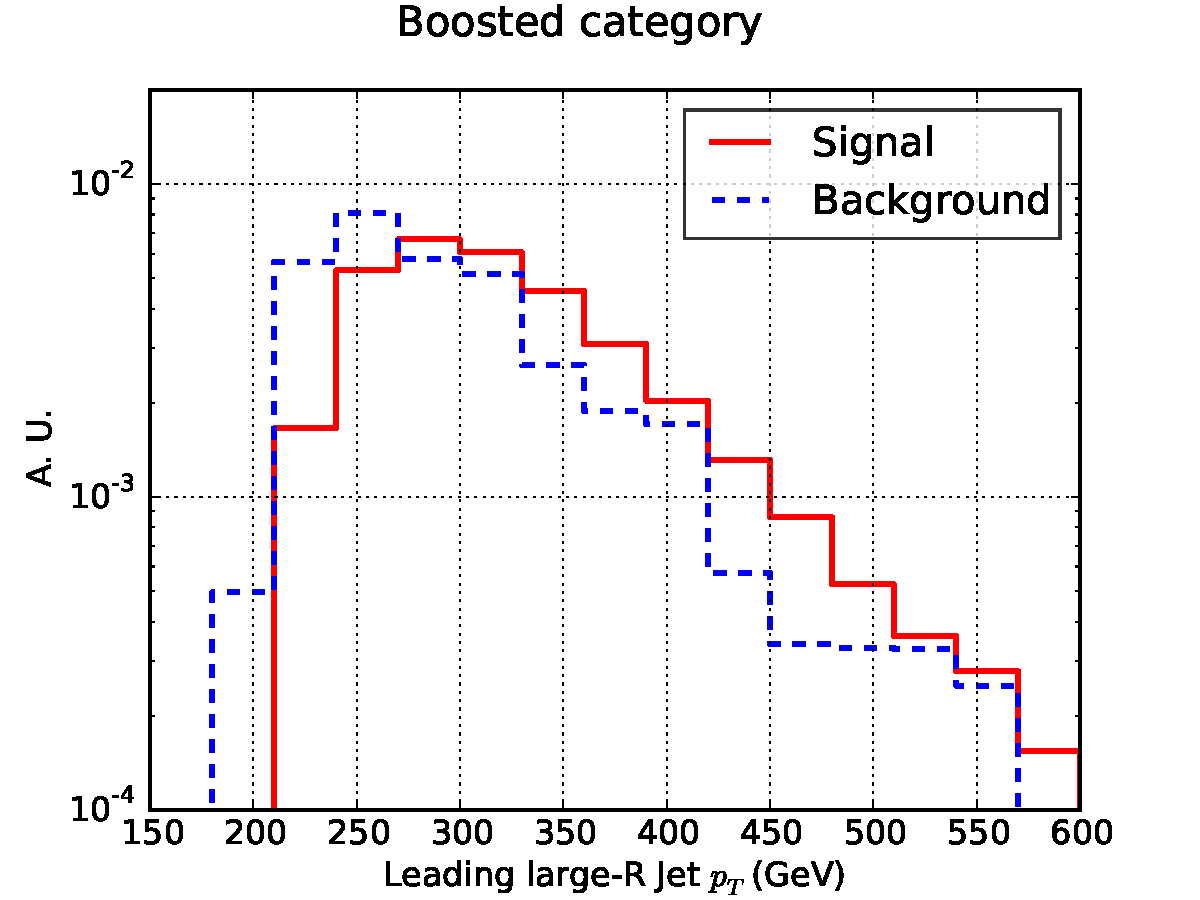
\includegraphics[width=0.48\textwidth]{plots/pt_H0_boost_C1.pdf}
 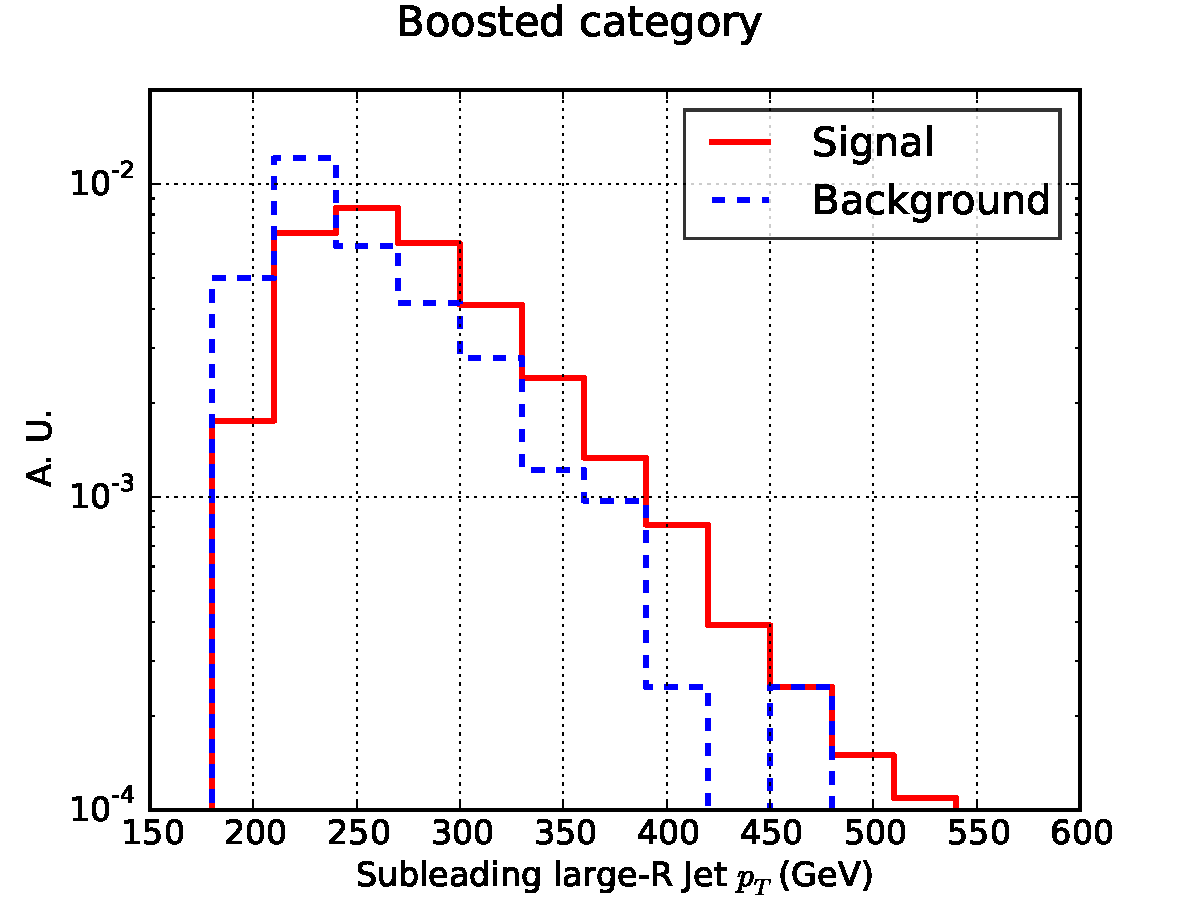
\includegraphics[width=0.48\textwidth]{plots/pt_H1_boost_C1.pdf}
\caption{\small  The $p_T$ distribution of the
  leading (left plot) and
  subleading (right plot) large-$R$ jets in the boosted category.
  %
  We comparing
  the shapes of the distribution in signal and background events,
  where both
  distributions have been normalized to their total integral.
}
\label{fig:cutplots1}
\end{center}
\end{figure}
%%%%%%%%%%%%%%%%%%%%%%%

{\bf Add missing plots here: pt of subjets(boosted), pt of
  small-R jets (resolved), rapidity of the large-$R$ jets,
rapidity of the small-$R$ jets.}


In the boosted category we require the two
leading subjets of the large-$R$ jet to be relatively
hard, in particular that should satisfy $p_T \ge $ 50 GeV.
%
To motivate this cut, in FigAAA
we show the distribution in $p_T$ of the leading
and subleading sub-jets in the leading large-$R$ jet in events
of the boosted category.
%
It is clear from the comparison that the subjet $p_T$ spectrum is
relatively harder in the signal with respect to the background,
motivating our choice of subjet $p_T$ cut.

In the resolved category,
it is important to understand the $p_T$ distribution
of the four leading small-$R$ jets of the event.
%
As noted in~\cite{deLima:2014dta}
given that in general the boost from the Higgs decays is moderate,
the two subleading jets might be not too hard, and thus it
should be important to ensure that our $p_T^{\rm min}$ cut
is not too strong.
%
This also has important implications for the experimental
trigger requirements in this category.
%
In Fig. we show the distribution in $p_T$ of the four leading
small-$R$ jets in signal and background events.
%
We see that the third and four leading jets are relatively soft.
%
Therefore, we can conclude that....


Another important distribution is the rapidity of the large-$R$
(in the boosted category) and the small-$R$ (in the resolved
category) jets.
%
We want to understand by how much the signal efficiency is reduced
by the restriction of the central region, and how would
the signal yield be enhanced if tracking could be extended
to forward rapidities in ATLAS and CMS.
%
Also, it is useful to show the distribution in rapidity of the
individual jets in the resolved category.
%
This comparison is shown in FigAAA.




Next, in Fig.~\ref{fig:mHHinv} we show the invariant mass
of the leading reconstructed Higgs candidates, before the Higgs mass window
cut Eq.~(\ref{higgsmasswindow})
  is applied, for the resolved and boosted categories.
%
The signal distribution is of course peaked at the
nominal Higgs mass of $m_h=125$ GeV.
%
In the boosted category, the background shows no particular
structure, while remarkable in the resolved category the background
also shows a peak-like structure, artificially induced by the
acceptance kinematical cuts on the jets.
%
Note that the applied smearing, which mimics detector resolution effects,
leads to a rather broad distribution which reduces the usefulness
of the Higgs mass window cut.
%
While our Higgs mass window cut is relatively loose,
information of the different shape of the $m_{h}$
distribution will still be exploited by the MVA.
%
In Sect.~\ref{sec:optimisation} we discuss how the results
of the analysis is modified if a more aggressive
detector resolution is assumed (corresponding
to a smaller value of the smearing).

%%%%%%%%%%%%%%%%%%%%%%%%%%%%
\begin{figure}[t]
\begin{center}
  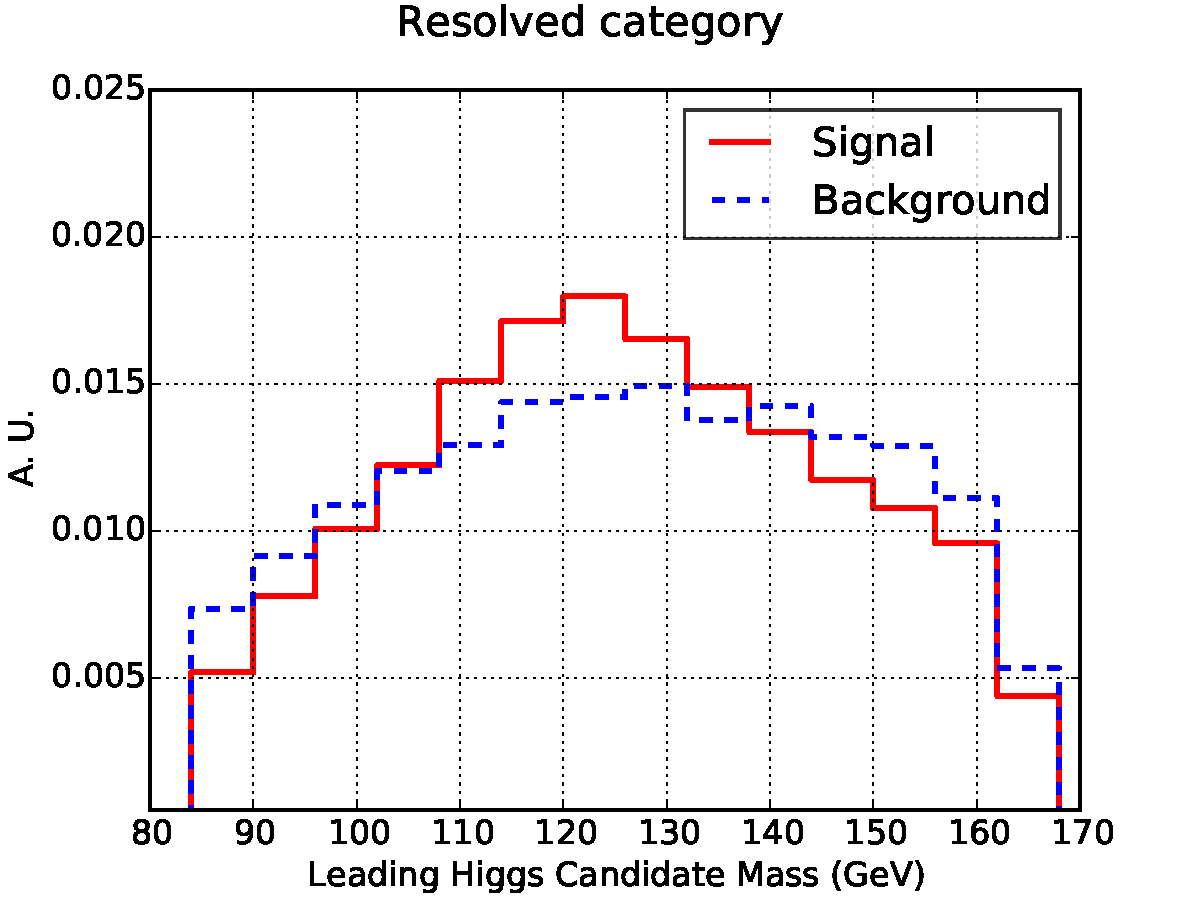
\includegraphics[width=0.48\textwidth]{plots/m_H0_res_C1.pdf}
  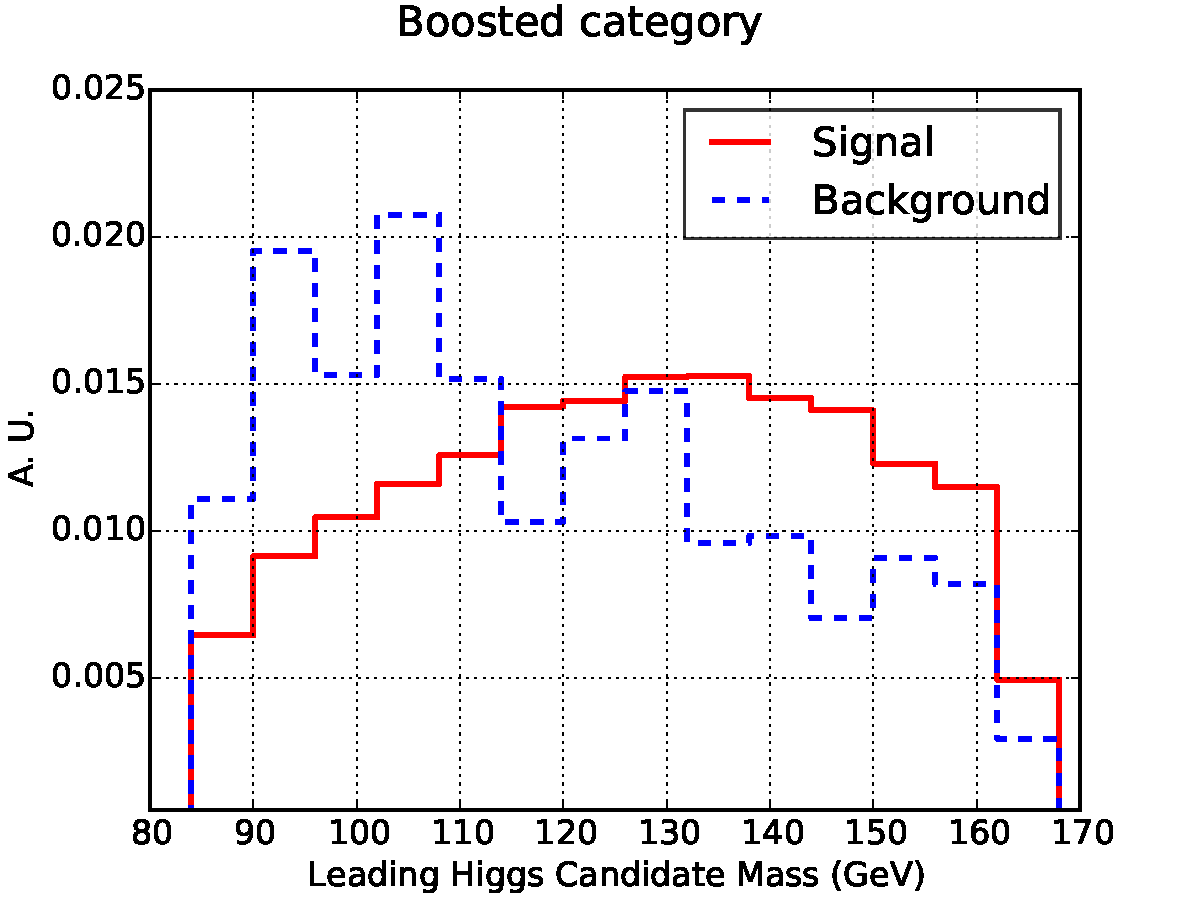
\includegraphics[width=0.48\textwidth]{plots/m_H0_boost_C1.pdf}
  \caption{\small The invariant mass distribution of the leading
    Higgs candidates on the resolved (left plot) and boosted (right
    plot) categories. {\bf redo boosted case with correct axes range}
}
\label{fig:mHHinv}
\end{center}
\end{figure}
%%%%%%%%%%%%%%%%%%%%%%%


Another important kinematical distribution of this process is the invariant mass
of the di-Higgs system.
%
First of all because this is a direct measure of the boost of the system,
and also because in many BSM scenarios this distribution can be substantially
modified as compared to the SM case, for example in the presence
of certain dimension-6 EFT operators~\cite{Azatov:2015oxa}.
%
Indeed, one important advantage of the $4b$ final state for
di-Higgs production is that it significantly increases the reach
in $m_{hh}$ as compared to other channels with smaller branching rations,
such as $2b2\gamma$.
%
With this motivation, we show in
Fig.~\ref{fig:mhh} the invariant mass distribution of the
reconstructed Higgs pairs,
comparing the resolved category (left) with the boosted category (right).


In the resolved case, we see that the distribution
in $m_{hh}$ is rather harder for the signal as for the background,
and thus one expects that cutting in $m_{hh}$ would help signal
discrimination: we will verify this with the help of the MVA.
%
For the boosted category the trend of the $m_{hh}$ distribution
is different because of the jet selection cuts, with the
distribution now peaking at higher values.
%
In this case signal and background distributions
look reasonably similar.
%
Note that at parton-level the $m_{hh}$ distribution as a kinematical
cut-off at $m_{hh}^{\rm min}=250$ GeV, which is modified by both
shower effects and by detector resolution effects.
%
While we don not cut in this quantity, it is
one of the inputs for the MVA to help to improve signal discrimination.

%%%%%%%%%%%%%%%%%%%%%%%%%%%%
\begin{figure}[t]
\begin{center}
  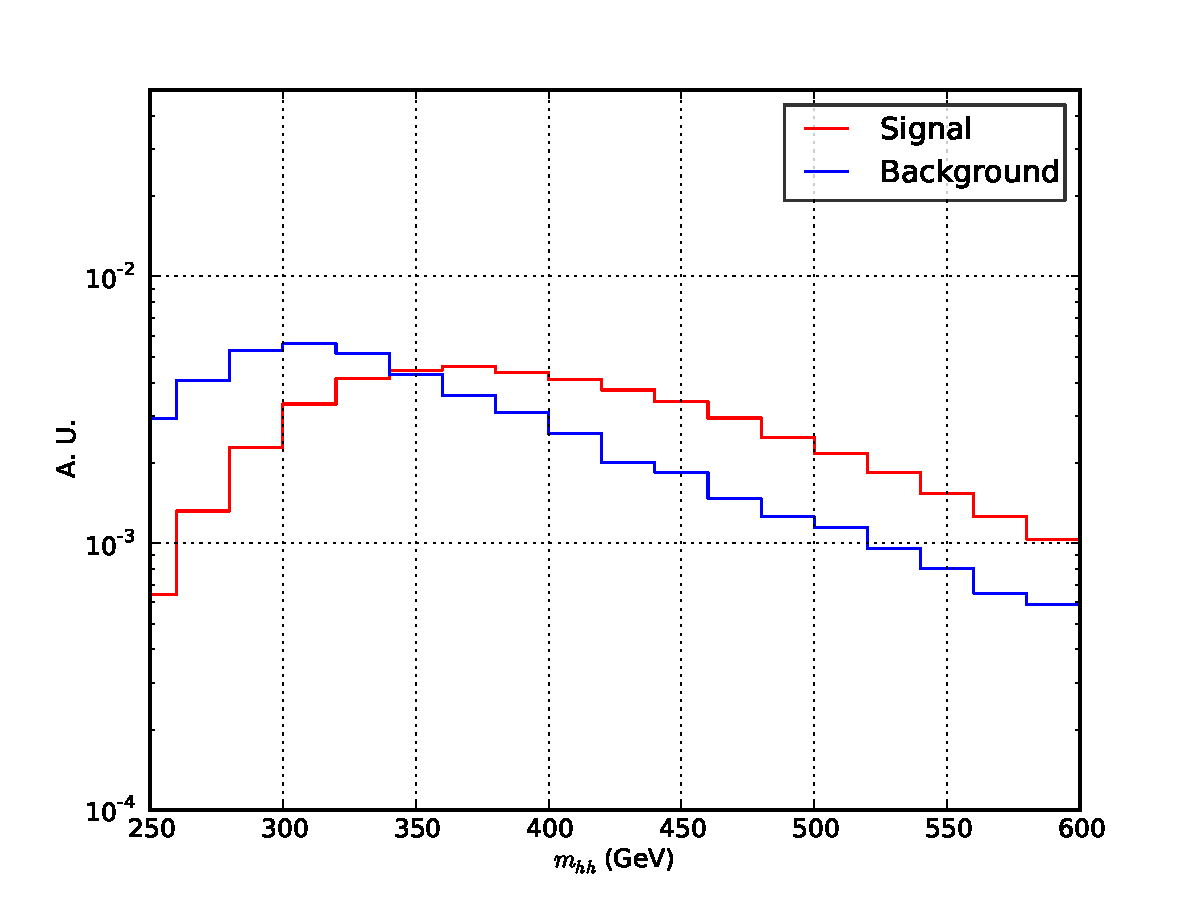
\includegraphics[width=0.48\textwidth]{plots/m_HH_res_C1.pdf}
  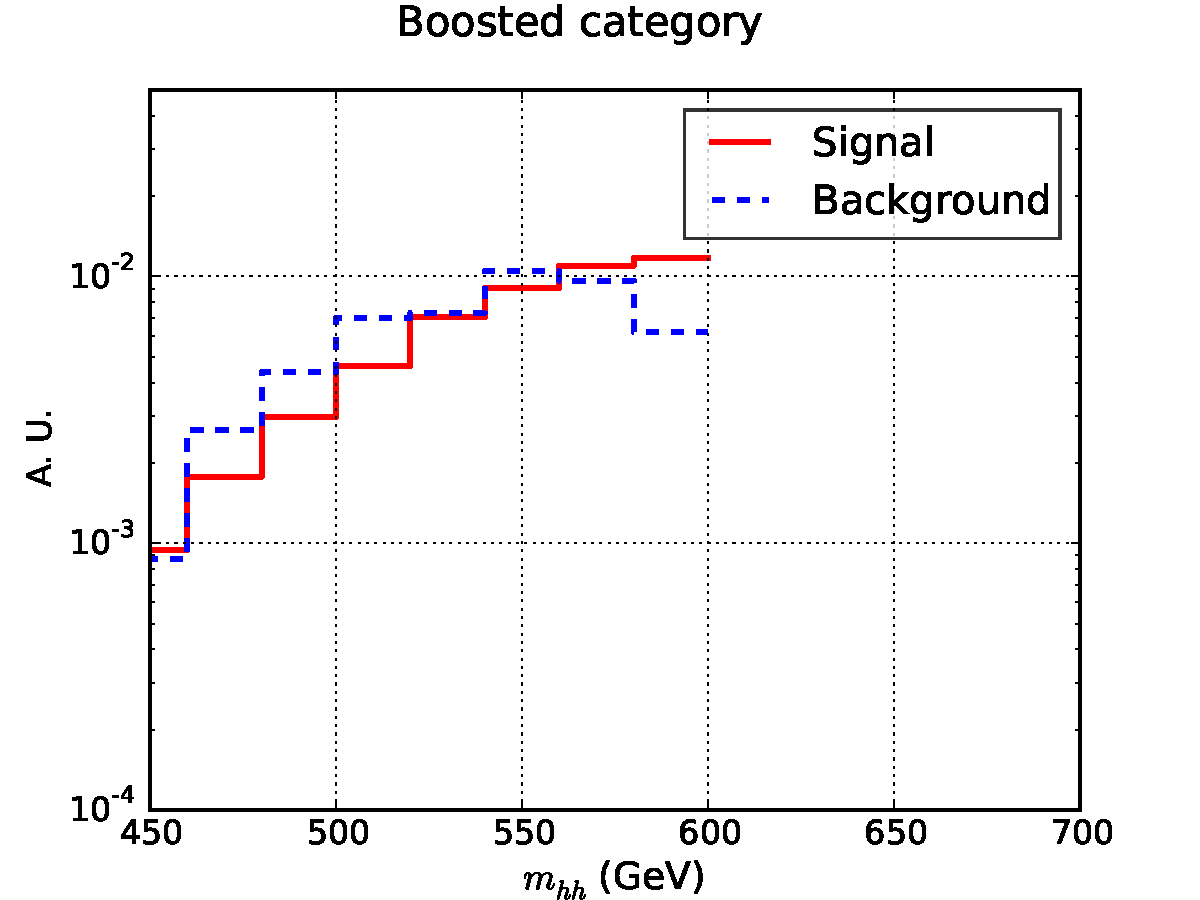
\includegraphics[width=0.48\textwidth]{plots/m_HH_boost_C1.pdf}
  \caption{\small Left plot: the invariant mass distribution of the Higgs
    pair candidates, $m_{hh}$, comparing signal and background events,
    in the resolved category.
    %
    Right plot: same for the boosted category.
}
\label{fig:mhh}
\end{center}
\end{figure}
%%%%%%%%%%%%%%%%%%%%%%%


Another interesting distribution is the transverse momentum of
the di-Higgs system.
%
In Fig.~\ref{fig:pthh} we show the $p_T^{hh}$
distribution
for the resolved and boosted categories.
%
Again we see that the background has a steeper $p_T^{hh}$ distribution
that the signal, in both categories, thus this variable
should provide some additional discrimination power, and therefore
we will use it as another of the MVA inputs.
%
Note that in our LO simulation this distribution is generated purely
by the parton shower - a more refined calculation would require
either the matching with higher-multiplicity matrix elements~\cite{Maierhofer:2013sha} or
the full NLO calculation~\cite{Frederix:2014hta}, to treat properly the first hard emission.
%
Nevertheless, the MVA shows only limited sensitivity to this variable, so its
modelling appears not to be crucial in our case.

%%%%%%%%%%%%%%%%%%%%%%%%%%%%
\begin{figure}[t]
\begin{center}
  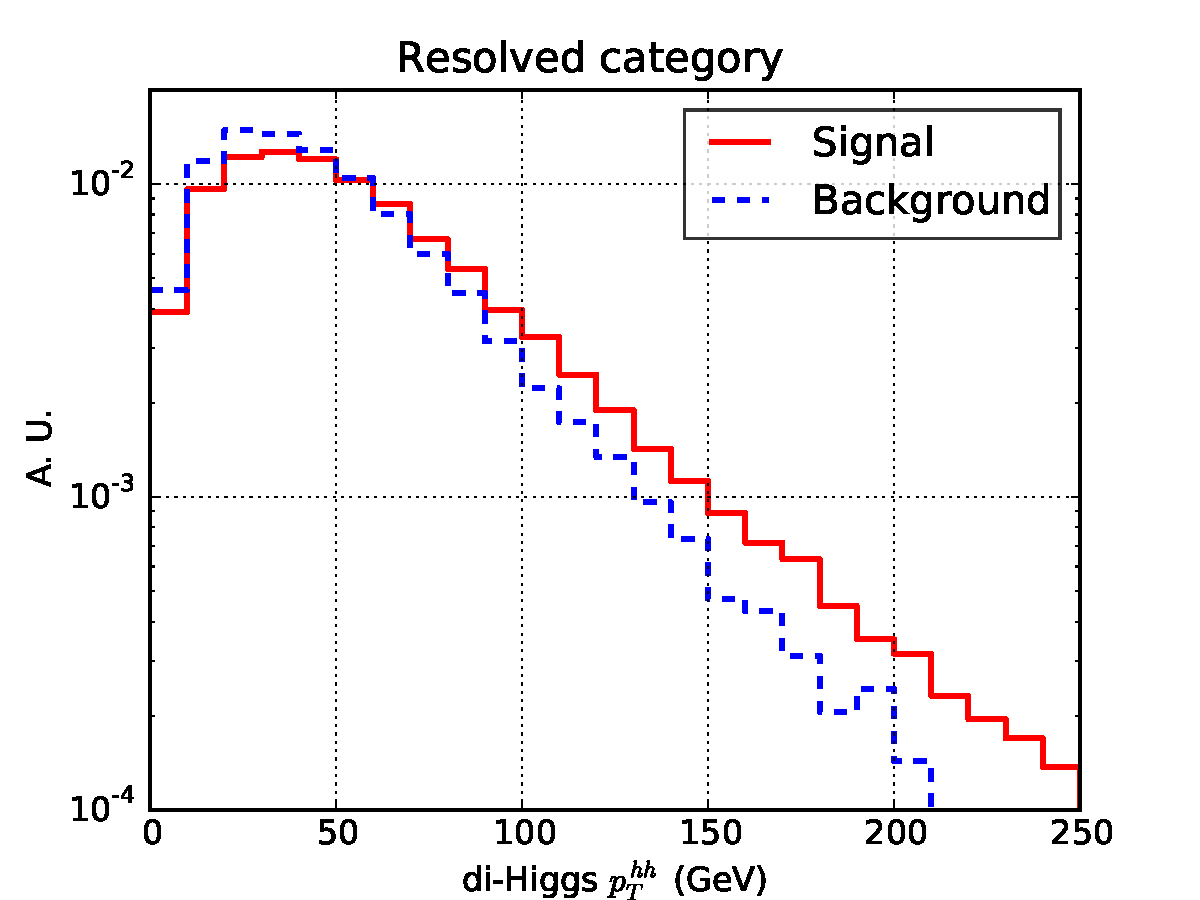
\includegraphics[width=0.48\textwidth]{plots/pt_HH_res_C1.pdf}
  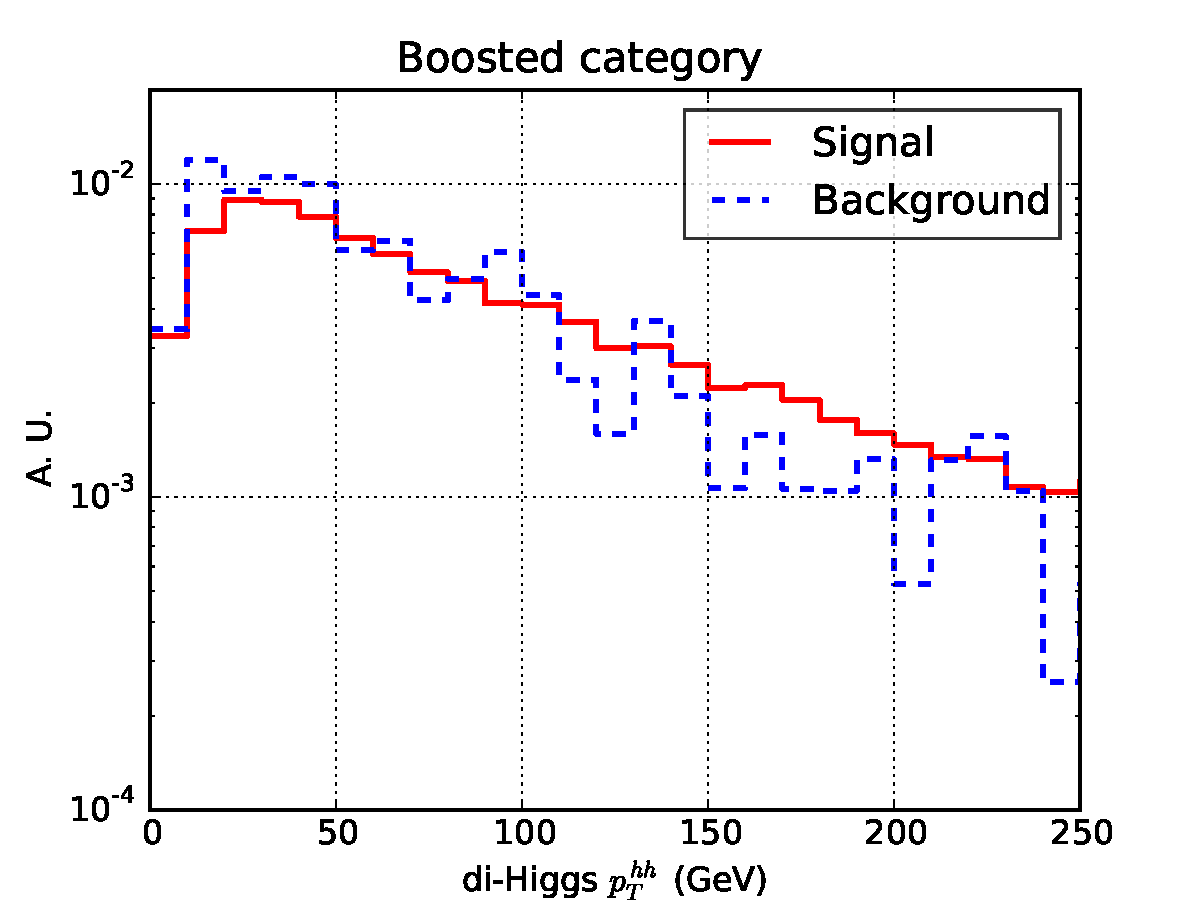
\includegraphics[width=0.48\textwidth]{plots/pt_HH_boost_C1.pdf}
  \caption{\small Same as Fig.~\ref{fig:mhh} for the transverse momentum
    distribution of the di-Higgs system $p_T^{hh}$.
}
\label{fig:pthh}
\end{center}
\end{figure}
%%%%%%%%%%%%%%%%%%%%%%%

